\section{概率体积：响应阶、任务阶与先验质量阶必须分开}
\label{sec:volume}

\subsection{单条相容路径不够定义概率体积}
一条高维材料空间中的光滑曲线通常具有零 prior 质量。由一条弧上的 $F(m(h))-F(m_0)\sim ch^p$，不能直接推出完整 posterior 的分支质量。必须建立一个有正测度的局部 chart/锥邻域，控制横向方向、角向零点、强变量条件积分、远分支和归一化。

同理，式 \eqref{eq:profile} 是几何补偿中心，不自动等于 noisy likelihood 的真正 profile 最优点，也不等于把强变量积分掉后的条件均值。若使用它作 Laplace 中心，须证明强 Hessian 稳定、局部唯一性及随噪声的余项控制；其 determinant/prior 体积因子不能丢。

\subsection{命题三：一个可严格证明的分层条件模型}
以下命题刻意限制到可验证模型，而不将一条 Maxwell 弧直接升级成 Full66 定理。

\begin{theorem}[任务分辨的接缝质量尺度]
\label{thm:scaling}
假设材料 prior 由 $m_0$ 的正质量原子 $w_0\delta_{m_0}$ 与一条真实一维材料分支组成。分支坐标 $h\in(0,h_0]$ 的 prior 为
$a(h)h^{\alpha-1}dh$，$a(h)\to a_0>0,\alpha>0$。固定噪声形状白化后
\[
\bar F(m(h))=\bar F(m_0)+c h^p+o(h^p),\quad c\ne0,
\]
\[
\varphi(m(h))-\varphi(m_0)=b h^s+o(h^s),\quad s\ge0.
\]
数据为 $\bar y=\bar F(m_0)+\sigma\xi$，$\xi$ 固定在一个有界集合中。假设缩放后的 evidence 被积函数与中心化任务被积函数分别具有统一可积支配；远离接缝的 evidence 贡献为 $o(\sigma^{\alpha/p})$，中心化任务贡献为 $o(\sigma^{(\alpha+s)/p})$；总归一化由原子项主导。则
\begin{align}
Z_{\rm br}(\sigma,\xi)
&=\sigma^{\alpha/p}\{a_0 I_{\alpha,p}(\xi)+o(1)\},\\
P({\rm br}\mid y)&=O(\sigma^{\alpha/p}),\\
T_\varphi(y)-\varphi(m_0)&=O(\sigma^{(\alpha+s)/p}),
\label{eq:three-exponents}
\end{align}
其中
\[
I_{\beta,p}(\xi)=
\int_0^\infty t^{\beta-1}
\exp[-\tfrac12\|ct^p-\xi\|^2]\,dt.
\]
若领先常数非零，$O$ 可加强为对应的渐近等价。典型分支宽度为 $h=O(\sigma^{1/p})$。
\end{theorem}
\begin{proof}
在分支 evidence 积分中令 $h=\sigma^{1/p}t$，测度因子变成
$\sigma^{\alpha/p}a(\sigma^{1/p}t)t^{\alpha-1}dt$，likelihood 逐点趋于定义中的指数函数。由统一支配与远分支控制可交换极限和积分。原子项为
$w_0e^{-\|\xi\|^2/2}$，有正的 $O(1)$ 极限，因此除以总 evidence 得分支质量阶。中心化任务分子额外乘 $b\sigma^{s/p}t^s+o(\sigma^{s/p})$，再除以同一归一化即可。
\end{proof}

对多维分支，可在极坐标下得到类似结果，但需要领先齐次响应在声明角域上统一非退化。例如 $w\in\R^d$，$\|P_p(w)\|\asymp\|w\|^p$，prior 径向指数为 $d+\beta-1$，则 $\alpha=d+\beta$。若强变量先积分，必须证明其 determinant、先验及正则噪声因子一致受控；不同 strata 的强方向维数不同会改变 evidence 的额外幂次。上述命题不能省略这些条件直接覆盖真实 Full66。

该命题使用成熟的奇异 Laplace 缩放思想。\refl{L15} 新颖性候选在于：用真实 Maxwell 补偿得到可验证的 $p$、有效局部域和常数，并区分材料任务的 $s$，而不是仅观察一个三次 decoder。

\subsection{R6 与真正 Maxwell 高阶弱性的区别}
\begin{longtable}{p{.29\linewidth}p{.19\linewidth}p{.2\linewidth}p{.24\linewidth}}
\toprule
局部机制 & $(p,s,\alpha)$ & 分支质量 & 材料任务漏项\\
\midrule
R6 三次 decoder seam，正原子主导 & $(3,3,1)$ & $\sigma^{1/3}$ & $\sigma^{4/3}$\\
材料正则弧，物理补偿至三阶，正原子主导 & $(3,1,1)$ & $\sigma^{1/3}$ & $\sigma^{2/3}$\\
事件跨分支跳变 & $(p,0,\alpha)$ & $\sigma^{\alpha/p}$ & 同阶 $\sigma^{\alpha/p}$\\
无原子、连续分支主导 & 同样的局部 $p,s$ & 可为 $O(1)$ & 通常条件变化尺度 $\sigma^{s/p}$\\
\bottomrule
\end{longtable}
第二行是条件理论，不是 R6 已证实的现象；真实 regular 材料 prior 通常并无 $m_0$ 原子，第四行往往更相关。对某个对称分支，材料均值的领先项还可能因奇偶性相消，均值误差很小而方差或事件仍大，因此同时评价均值、协方差和材料事件。

\begin{figure}[htbp]
\centering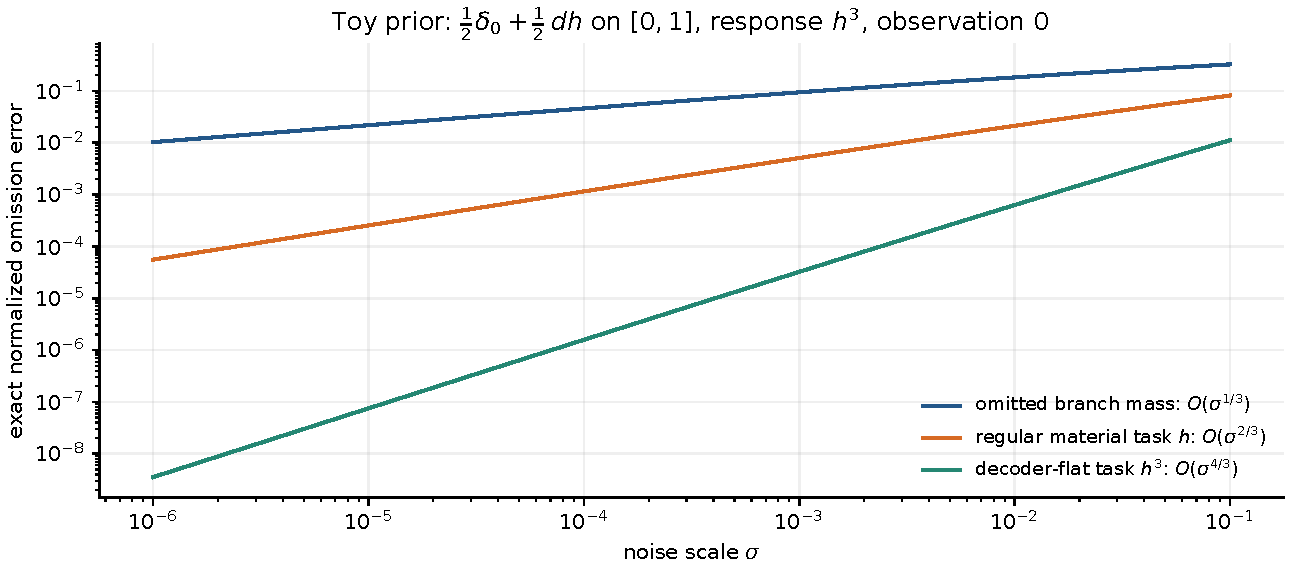
\includegraphics[width=.95\linewidth]{figures/atom_task_scaling.pdf}
\caption{正原子主导的受控一维模型。相同三阶响应下，分支质量、正则材料任务和 decoder 平坦任务有不同误差阶。图中是归一化积分的解析结果，不能外推为 Full66 或普通无原子材料先验的规律。}
\end{figure}

\subsection{三个阻止错误外推的反例}
\textbf{无原子。} $h\sim\mathrm{Uniform}[0,1]$，$F(h)=h^p$，观测零附近。posterior 全部位于连续分支，分支概率恒为 1；只能说其宽度缩小。$\sigma^{1/p}$ 质量说法不成立。

\textbf{角向退化产生对数。} $(u,v)\sim\mathrm{Uniform}[0,1]^2$，$F=uv$。有
\[
P(uv\le\sigma)=\sigma+\sigma\log(1/\sigma),\quad0<\sigma<1.
\]
证明为分别积分 $u\le\sigma$ 和 $u>\sigma$ 时允许的 $v$ 长度。一条固定方向的二阶响应，不能捕获靠近坐标轴的体积与对数因子。

\textbf{固定离开模型的 residual。} 若观测与所有局部响应保持不随 $\sigma$ 缩小的偏离，likelihood 可能由边界、远分支或另一鞍点主导；固定标准化创新假设失效。不能把一个局部 seam 的小噪声公式解释为全局 posterior 率。

\subsection{真正必要的体积是什么}
需要计算的是对任务积分有影响的 $L_y\,d\mu_0$，以及漏掉区域的可控贡献。若只求一个有界材料功能，不必恢复每个 latent 的联合 density；若要多个物理模式的概率、置信区域或主动测量，必须知道不同材料分支的质量；若报告“latent $Q>0.5$”这样的非材料事件，还必须保留 $K_G$。不存在对所有任务都可以删除的“无用概率体积”。

\section{Task-Conditional Observability：一个一阶响应和一个完整任务信息对象}
\label{sec:taskinfo}

\subsection{不要把敏感性、剩余风险和新增信息混成一个量}
对向量任务 $\varphi(M)$，至少有三个对象：
\[
T_\varphi(y)=\E[\varphi\mid y],\qquad
V_\varphi(y)=\Cov(\varphi\mid y),\qquad
D_yT_\varphi(y).
\]
第一个是估计，第二个是条件不确定性，第三个是对当前数据的局部响应。高敏感性不意味着大风险下降；零导数也不意味着完全无信息。对于新采集 $a$，真正的实验信息还涉及尚未见到的 $Y_a$。

\subsection{Gaussian 任务响应及层内/层间分解}
在允许微分与积分交换的可积条件下，经典 Gaussian identity 给出
\begin{equation}
D_yT_\varphi(y)=
\Cov(\varphi(M),F(M)\mid y)\Gamma^{-1}.
\label{eq:task-score}
\end{equation}
由求导归一化 likelihood 可直接证明：score 是
$\Gamma^{-1}(F(M)-\E[F\mid y])$，与 $\varphi$ 相乘再取期望即可。它允许材料原子，不要求 prior 有 Lebesgue density；这已被一般 conditional-mean identity 覆盖。\refl{L17}

定义一阶白化任务响应
\[
B_\varphi(y)=\Cov(\varphi,F\mid y)\Gamma^{-1/2}.
\]
对互斥的材料分支标签 $S$，
\[
\Cov(\varphi,F\mid y)
=
\sum_s w_s\Cov_s(\varphi,F)
+
\Cov_{S\mid y}\big(\E[\varphi\mid S,y],\E[F\mid S,y]\big).
\]
第一项是分支内响应，第二项是分支质量迁移的代数贡献。向量或矩阵的两项通常不正交，范数比例不构成可加的信息百分比。R6 的约 28\% 是 between-source 导数范数比；source 的材料像可重叠，因此更不能直接称为 28\% 的物理模式信息。\refe{R6-A}

在局部线性 Gaussian 近似，$\varphi\approx Lm$，
\[
B_\varphi\approx L C_{\rm post}J^*\Gamma^{-1/2}.
\]
任务相关方向由 $L$、posterior covariance、$J$ 及噪声共同决定，不只是 $J^*J$ 的最大特征向量。此基本原则已有 goal-oriented inverse 的最优低秩理论。\refl{L7}

\subsection{命题四：完整的新增测量任务信息}
令当前 posterior 为 $\mu_y$，新采集的条件分布为 $p_a(dz\mid m)$。定义中心化条件期望算子
\[
\mathcal C_{a,y}:L^2_0(\mu_y)\longrightarrow L^2_0(p_a(\cdot\mid y)),
\quad
g\longmapsto \E[g(M)\mid y,Y_a].
\]
其任务信息算子为
\[
\mathcal O_{a,y}=\mathcal C_{a,y}^*\mathcal C_{a,y}.
\]
这是真正作用于材料函数的算子，不必把材料函数线性化成一个方向。

\begin{theorem}[任务信息与 Bayes 风险；成熟条件期望原理]
\label{thm:task-information}
$\mathcal O_{a,y}$ 自伴、半正定，且 $0\preceq\mathcal O_{a,y}\preceq I$。对标量平方任务，
\begin{align}
\langle\varphi-\E_y\varphi,\mathcal O_{a,y}(\varphi-\E_y\varphi)\rangle
&=\Var_{Y_a\mid y}\big(\E[\varphi\mid y,Y_a]\big)\\
&=\Var(\varphi\mid y)-\E_{Y_a\mid y}\Var(\varphi\mid y,Y_a).
\label{eq:task-bayes-reduction}
\end{align}
向量任务的对应矩阵
$\mathcal I_{a,\varphi}(y)=\Cov_{Y_a\mid y}(\E[\varphi\mid y,Y_a])$
为平均后验任务 covariance 的精确下降。
\end{theorem}
\begin{proof}
条件 Jensen 给 $\|\mathcal C g\|_2\le\|g\|_2$，故 $\mathcal C^*\mathcal C$ 是正收缩。第一等式来自算子定义；第二等式为条件全方差公式。向量情形逐个二次型应用标量结果。
\end{proof}

该算子可以称为本问题的 task-information 对象，但不能宣称它独立于成熟 Bayesian decision theory。它的 Maxwell 特征全部进入 $p_a(dz\mid m)$ 和 $\mu_y$。可能的新贡献是利用真实物理补偿结构计算它，而不是给它取名。

如果新增观测重复旧响应且噪声趋零，它无法区分旧 exact fibers 内的材料。新采集沿旧 fiber 变化，才可能降低给定旧无噪响应后的材料任务方差；对指定平方任务，平均风险严格下降当且仅当相应条件任务均值随新增观测非恒定。单次观测的 posterior 方差不保证下降。材料可区分性与任务条件依赖共同连接多解探索和测量设计。\refl{L18,L19}

\subsection{一阶协方差不是完整的信息：精确反例}
设当前材料只有三个值，
\[
M\in\{-1,0,1\},\qquad P=(1/4,1/2,1/4),\qquad
\varphi(M)=M^2,
\]
新观测为 $Y_t=\sqrt tM+N$，$N\sim N(0,1)$。因为对称性，
$\Cov(M^2,M)=0$。但
\[
\E[M^2\mid Y_t=z]
=
\frac{e^{-t/2}\cosh(\sqrt t z)}
{1+e^{-t/2}\cosh(\sqrt t z)}
\]
对每个 $t>0$ 都不是常数，所以真正任务信息严格为正。展开得
\[
\E[M^2\mid Y_t=z]=
\tfrac12+\tfrac{t}{8}(z^2-1)+O(t^2),
\qquad
\mathcal I_{t,\varphi}=\frac{t^2}{32}+o(t^2).
\]
以上点态展开配合 Gaussian 可积余项控制给出方差渐近。这说明零一阶协方差不能断言任务无信息。对新采集
$Y_{a,t}=\sqrt t F_a(M)+\eta_a$，$\eta_a\sim N(0,\Gamma_a)$，
新增噪声条件于材料与旧数据独立。定义
\[
B_{a,\varphi}(y)=\Cov_{\mu_y}(\varphi,F_a)\Gamma_a^{-1/2}.
\]
在相应矩与微分条件下，
$\mathcal I_{a,t,\varphi}=tB_{a,\varphi}B_{a,\varphi}^*+o(t)$。
这里使用新采集而非旧 $F$ 的协方差。上述对称例的一阶项为零，必须保留更高阶或有限信号模型；若新增噪声与旧数据相关，应使用完整条件通道 $p_a(dz\mid m,y)$。

\begin{figure}[htbp]
\centering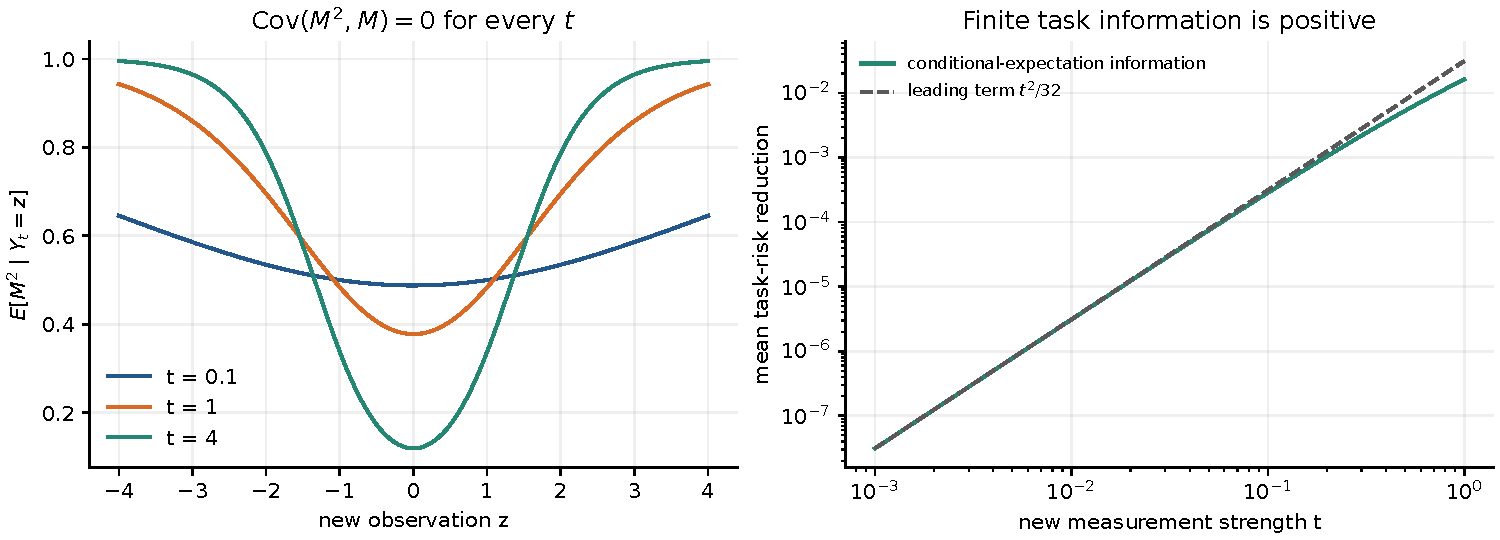
\includegraphics[width=\linewidth]{figures/zero_covariance_information.pdf}
\caption{三点材料先验的解析反例：一阶任务协方差为零，但新观测对平方任务的信息严格为正。右图为一维 Gaussian 求积与小信号公式；未运行 Maxwell。}
\end{figure}

\subsection{为什么不合格 posterior provider 仍能改善材料成像}
平方损失的标准分解为
\[
\E\|\widehat a(Y)-M\|^2
=
\E\|T_M(Y)-M\|^2+
\E\|\widehat a(Y)-T_M(Y)\|^2.
\]
一个 provider 即使不能给出正确联合密度，也可能输出与 $T_M$ 有关的有用特征；下游监督 head 可使用这些特征降低第二项。R4 的普通 Gaussian 与 Flow 融合几乎同样好，符合这种解释，但没有测到真正的 $T_M$，不能从现有数据精确分解其 Bayes excess。

进一步，posterior mean 通常不在 decoder image 内。要求 Maxwell-consistent representative 时，可以在可行材料中求
\[
m_{\rm rep}\in\argmin_{m\in\mathcal A(y)}
\E_{\mu_y}\|m-M\|_{W_M}^2,
\]
等价于在所声明的可行集合 $\mathcal A(y)$ 中投影 posterior mean；这与均值、MAP、样本是不同输出。$\E F(M)\ne F(\E M)$ 也意味着均值图散射不相容未必说明条件均值错误。

\subsection{物理特征的计算价值不等于新增观测信息}
固定已知 forward、prior 和训练资产，若 current、Jacobian、KKT 或其它特征为 $A(Y)$，则
\[
\sigma(Y,A(Y))=\sigma(Y),\qquad
\E[\varphi(M)\mid Y,A(Y)]=\E[\varphi(M)\mid Y].
\]
第一式直接来自 $A(Y)$ 的可测性，第二式来自条件期望的唯一性。引入条件于 $Y$ 独立于材料的算法随机种子，也不会增加真实材料信息。这是数据处理原则的直接应用，不是新的 Maxwell 定理。

因此 E5 所谓“超出 raw measurement 的增量”只能指：有限数据、有限容量、有限训练或有限物理预算下，材料统计更容易被估计，或者达到同一精度更便宜；不能声称确定性物理特征增加了原始数据的 Shannon 信息。若另有新采集、未知模型校准或外部 prior 信息，须显式加入观测/条件模型。

这一区别同样适用于任务导向物理计算：继续计算 current 或 Jacobian 可以降低已有材料信息的数值提取误差，真实新增采集则可能减少材料的统计不确定性。两种费用可以联合优化，但不是同一种信息增益。

\subsection{没有合格 Full posterior sampler 时如何估计}
可以采用三条有不同资格的路径。

第一，在低维非均匀条件模型中用可信全域积分计算 $T,V,B,\mathcal I$，检验理论与误差，不把条件切片冒充 Full66 边缘。第二，利用 prior predictive 模拟对 $(Y,\varphi(M))$ 做 proper supervised regression，直接估计任务条件矩；这是风险学习，需独立任务 MSE 与事件校准，不能据此认证全部 posterior。第三，多中心局部 Gaussian/stratified mixture 可作计算近似，但权重、外部质量及高阶盲点均须单列。

R6 B6 的高 SNR 条件矩回归失败提示：原始矩相减再乘 $\sigma^{-2}$ 会放大回归误差。使用同 fold 的中心化目标、标准化观测、直接任务回归或双样本校正可以改善数值条件，但导数一致性仅是必要诊断之一；一个错误模型也可能内部自洽。\refe{R6-B}

材料均值、局部相事件、空腔事件、covariance、后验预测散射和工程功能量必须分别评价。均值很准不保证结构存在概率准；某个任务 covariance 小也不保证另一个非线性任务容易判断。

